%!TEX options=--shell-escape
\documentclass[tikz]{standalone}
\usepackage[T1]{fontenc}
\usepackage[utf8]{inputenc}
\usepackage{xcolor}
\usepackage{amsmath}
\usepackage{amssymb}
\usepackage{hyperref}
\usepackage{accsupp}    
\usepackage{graphicx}
\usepackage{mathtools}
\usepackage{pagecolor}
\usepackage{amsmath} % for \dfrac
\usepackage{tikz}
\tikzset{>=latex} % for LaTeX arrow head
\usepackage{pgfplots} 
\usepackage[edges]{forest}
\usetikzlibrary{patterns, backgrounds, arrows.meta}
\setlength{\parindent}{0cm}
\setlength{\parskip}{1em}
\usepackage{braket}

\usetikzlibrary{patterns}

\begin{document}
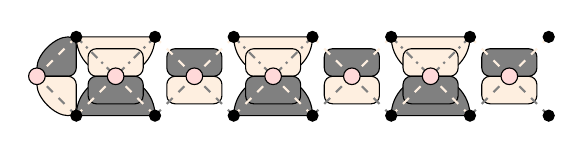
\begin{tikzpicture}[]

 \foreach \x in {0, 2,...,4}{
    \draw[black, fill=yellow!40!red!10](\x,1) arc (0:180:-0.5) -- cycle;
    \draw[black, fill=gray](\x,0) arc (180:0:0.5) -- cycle;
    } 

   \foreach \x in {0, 2,...,4}{
        \fill[draw=black, fill=yellow!40!red!10, rounded corners=3pt] (\x + 0.15, 0.5) rectangle (\x+0.85, 0.85) ;
        \fill[draw=black, fill=yellow!40!red!10, rounded corners=3pt] (\x + 1.15, 0.15) rectangle (\x+1.85, 0.5) ;
        \fill[draw=black, fill=gray, rounded corners=3pt] (\x + 0.15, 0.15) rectangle (\x+0.85, 0.5) ;
        \fill[draw=black, fill=gray, rounded corners=3pt] (\x + 1.15, 0.5) rectangle (\x+1.85, 0.85) ;


    }
    \fill[draw=black, fill=gray, rounded corners=3pt] (-0.5, 0.5) -- (0, 0.5)  -- (0, 1) arc (90:180:0.5) -- cycle ;
    \fill[draw=black, fill=yellow!40!red!10, rounded corners=3pt] (-0.5, 0.5) -- (0, 0.5)  -- (0, 0) arc (270:180:0.5) -- cycle ;

    \foreach \x in {0, 2, ..., 4}{
           \draw[thick, dashed, yellow!40!red!10] (\x, 0) -- (\x + 0.5, 0.5);
           \draw[thick, dashed, yellow!40!red!10] (\x+1, 0) -- (\x + 0.5, 0.5);

           \draw[thick, dashed, gray] (\x+1, 0) -- (\x + 1.5, 0.5);
           \draw[thick, dashed, gray] (\x+2, 0) -- (\x + 1.5, 0.5);

           \draw[thick, dashed, yellow!40!red!10] (\x+1, 1) -- (\x + 1.5, 0.5);
           \draw[thick, dashed, yellow!40!red!10] (\x+2, 1) -- (\x + 1.5, 0.5);

           \draw[thick, dash dot, gray] (\x, 1) -- (\x + 0.5, 0.5);
           \draw[thick, dash dot, gray] (\x+1, 1) -- (\x + 0.5, 0.5);

    }
   \draw[thick, dashed, yellow!40!red!10] (0, 1) -- (-0.5, 0.5);
   \draw[thick, dashed, gray] (0, 0) -- (-0.5, 0.5);

    \foreach \x in {0, 1, ...,6}{

           \filldraw[draw=black, fill=black] (\x, 0) circle[radius=2pt] node[font=\tiny] {};
           \filldraw[draw=black, fill=black] (\x, 1) circle[radius=2pt] node[font=\tiny] {};
           \filldraw[draw=black, fill=pink!60] (\x - 0.5, 0.5) circle[radius=3pt] node[font=\tiny] {};
    }

\end{tikzpicture} 
\end{document}

